\chapter{Stand der Technik: Cyber-Range-Plattformen}
\label{chap:stand-der-technik}

Cyber Ranges werden in der Literatur für unterschiedliche Zwecke eingesetzt. Für das vorliegende Vorprojekt steht jedoch nicht die
Durchführung von Capture-the-Flag-(CTF)-Formaten oder der Einsatz kommerzieller
Trainingsplattformen im Vordergrund. Ziel ist vielmehr die Identifikation einer
selbst betreibbaren Plattform, die als Forschungsumgebung genutzt werden kann
und damit insbesondere Anforderungen wie Reproduzierbarkeit, Automatisierung und
Tool-Integration unterstützt.

Diese Fokussierung führt dazu, dass viele verbreitete Lösungen bewusst ausgeschlossen werden:
CTF- ausgerichtete Umgebungen sind häufig nicht darauf ausgelegt,
komplexe Infrastrukturzustände reproduzierbar bereitzustellen und externe Sicherheits- oder
Monitoring-Werkzeuge systematisch in UseCases einzubinden. Kommerzielle Plattformen sind
zudem meist nicht transparent genug, um sie als Forschungsumgebung zu
verwenden (z.\,B. fehlender Quellcodezugang). Im Ergebnis bleibt eine vergleichsweise kleine Menge an
Open-Source-Ansätzen übrig, die für den Aufbau einer forschungsorientierten Cyber Range
realistisch in Frage kommen.


\section{Anforderungen an Cyber Ranges für Forschungszwecke}
\label{sec:anforderungen-forschung}

Aus Forschungsperspektive lassen sich an eine Cyber Range Anforderungen ableiten, die über
klassische Trainingsfunktionen hinausgehen. Zentrale Voraussetzung ist die Fähigkeit, identische
Szenarien unter kontrollierten Randbedingungen wiederholt auszuführen, um Ergebnisse zwischen
Werkzeugen, Konfigurationen oder Methoden vergleichbar zu machen. Reproduzierbarkeit umfasst
dabei sowohl die technische Bereitstellung (Infrastruktur, Netzwerksegmente, Systeme, Rollen, ...)
als auch die Nachvollziehbarkeit des Szenarioablaufs und der Messpunkte.

Eng damit verbunden ist ein hoher Automatisierungsgrad. Für eine forschungsorientierte Nutzung
müssen Szenarien und Umgebungen möglichst einfach beschrieben und automatisiert ausgerollt
werden können (z.\,B. Infrastructure-as-Code). Darüber hinaus ist Erweiterbarkeit wesentlich: Die Plattform sollte so aufgebaut sein, dass neue Szenarien, zusätzliche Messpunkte oder Integrationen (z.\,B. Log- und Telemetriequellen) am Gesamtsystem möglich sind. Zur Erhebung und Auswertung von Messdaten werden in modernen IT-Umgebungen häufig Observability-Stacks eingesetzt,
z.\,B.\ Prometheus und Grafana für Metriken und Visualisierung sowie OpenTelemetry als Standard zur Instrumentierung
und zum Export von Telemetriedaten. Für zentrale Log-Auswertung werden häufig Elastic Stack oder Grafana Loki genutzt.


Ein weiteres Kernkriterium ist die Integrationsfähigkeit externer Werkzeuge. Da die Masterarbeit
später konkrete Cyber-Resilienz-Use-Cases umsetzen und evaluieren soll, muss die Cyber Range
Schnittstellen für Monitoring, Detection und Auswertung unterstützen. Resilienzbezogene Untersuchungen setzen zudem voraus, dass Systemverhalten über Zeit beobachtet und bewertet werden kann, was eine geeignete Beobachtbarkeit (Logging, Metriken, Events) voraussetzt.

Schließlich sind Betrieb und Governance zu berücksichtigen: Eine Forschungsumgebung muss
isoliert und sicher betrieben werden können, Mehrbenutzerbetrieb unterstützen und dabei
Rollen- und Zugriffsmodelle abbilden. Für das Vorprojekt sind außerdem Faktoren wie
Dokumentationsqualität, Community-Aktivität, Lizenzmodell und der Bereitstellungsaufwand relevant, da sie Machbarkeit der späteren Umsetzung stark beeinflussen.


\section{Analyse ausgewählter Open-Source-Cyber-Ranges}
\label{sec:analyse-open-source}

Auf Basis der genannten Anforderungen werden im Folgenden ausgewählte Open-Source-Ansätze
betrachtet, die grundsätzlich selbst betrieben und für Forschungsszenarien angepasst werden
können. Der Fokus liegt auf Plattformen, die nicht nur einzelne Trainingslabore bereitstellen,
sondern Funktionen zur Szenariobeschreibung, automatisierten Bereitstellung und
Umgebungssteuerung unterstützen.

\subsection{KYPO}
\label{subsec:kypo}

KYPO ist eine Open-Source-Cyber-Range-Plattform aus dem akademischen Umfeld, mit der sich
isolierte IT-Umgebungen für Übungen und Experimente bereitstellen und verwalten lassen.
Im Zentrum steht das Konzept von Sandboxes: vordefinierte Umgebungen, die bei Bedarf
bereitgestellt, genutzt und anschließend wieder zurückgesetzt oder entfernt werden können.
Die aktive Weiterentwicklung von KYPO CRP wurde inzwischen eingestellt; als Nachfolgeplattform wird CyberRangeCZ genannt \cite{KYPOConceptualArchitecture}.

\begin{figure}[H]
    \centering
    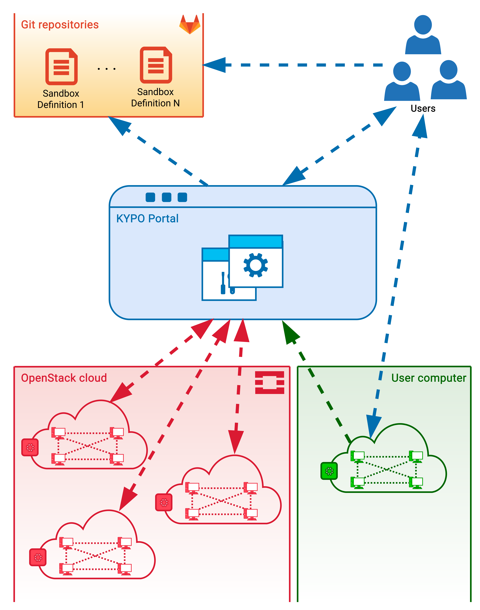
\includegraphics[width=0.7\linewidth]{kypo.png}
    \caption{Konzeptionelle Architektur von KYPO - Quelle: \cite{KYPOConceptualArchitecture}}
    \label{fig:kypo-conceptual-architecture}
\end{figure}

Abbildung~\ref{fig:kypo-conceptual-architecture} zeigt die Grundidee von KYPO in vereinfachter Form:
\emph{Sandbox-Definitionen} werden in Git-Repositories versioniert abgelegt. Das \emph{KYPO Portal}
dient als zentrale Komponente für die Verwaltung und nutzt diese Definitionen, um die
entsprechenden Ressourcen in einer \emph{OpenStack-Cloud} bereitzustellen. Nutzer greifen anschließend
von ihren Endgeräten auf die erzeugten Sandboxes zu.

Aus funktionaler Sicht übernimmt KYPO damit insbesondere (1) die Verwaltung von Sandbox-Definitionen
und deren Versionierung über Git, (2) die Orchestrierung und Bereitstellung der Umgebungen in OpenStack
sowie (3) den Zugang und die Nutzung der bereitgestellten Umgebungen durch Benutzer über das Portal.

\subsection{CyberRangeCZ}
\label{subsec:cyberrangecz}

CyberRangeCZ ist eine Open-Source-Plattform zur Erstellung und 

szenariobasierter Cyber-Range-Übungen mit dynamischer Bereitstellung von isolierten
Umgebungen (\emph{Sandboxes}). Die Plattform wird als Weiterentwicklung der KYPO Cyber
Range Platform (KYPO CRP) beschrieben und baut konzeptionell auf deren Ansatz auf,
während die technische Umsetzung stärker auf moderne, containerisierte Komponenten
und automatisierbare Bereitstellung ausgerichtet ist \cite{CyberRangeCZCyberRanges,CyberRangeCZGitHub}.

Aus architektonischer Sicht wird CyberRangeCZ als containerbasierte Microservices-Plattform
dargestellt. Zentrale Bausteine sind dabei insbesondere ein Sandbox Service zur
Lebenszyklusverwaltung der bereitgestellten Umgebungen sowie Trainingsdienste für
lineare und adaptive Trainingspfade (inklusive Unterstützung für Feedback- und
Auswertungsfunktionen) \cite{CyberRangeCZGitHub}.
Die Bereitstellung der Workloads erfolgt laut Projektbeschreibung auf einer
Kombination aus Kubernetes und Cloud-Backends, wobei u.\,a. OpenStack und AWS als
Zielumgebungen genannt werden \cite{CyberRangeCZGitHub}.

Ein wesentliches Merkmal der Plattform ist, dass die Bereitstellung und Konfiguration
stark automatisierungsorientiert beschrieben wird. In den Repositories finden sich dazu
u.\,a. Artefakte und Deploymentskripte, die auf gängigen IaC- und Cluster-Mechanismen
aufbauen (z.\,B. Helm-basierte Deployments), wodurch sich Installationen und Umgebungen strukturiert
wiederholbar aufsetzen lassen \cite{CyberRangeCZGitHub,CyberRangeCZDocs}.

Für den praktischen Betrieb stellt CyberRangeCZ ein webbasiertes Portal zur Verfügung,
über das Benutzer und Trainings verwaltet und Sandboxes gestartet werden können.
Szenarien bzw.\ Trainingsdefinitionen werden als wiederverwendbare Artefakte gepflegt,
wodurch sich Konfigurationen versionieren und iterativ anpassen lassen \cite{CyberRangeCZGitHub}.
Darüber hinaus wird die Plattform explizit als Grundlage genannt, um externe
Werkzeuge in Übungen einzubinden bzw.\ Übungen so zu gestalten, dass eine Integration
mit Drittanbietertools möglich ist \cite{CyberRangeCZCyberRanges}. Neben der technischen Dokumentation ist die Plattform auch über öffentliche
Entwicklungs- und Austauschkanäle nachvollziehbar: Quellcode, Issue-Tracking und
Diskussionen sind zentral über die Projektorganisation gebündelt.
\cite{CyberRangeCZGitHub}.

\subsection{Open Cyber Range (OCR)}
\label{subsec:ocr}

Open Cyber Range (OCR) ist ein Open-Source-Ansatz zur Erstellung und zum Betrieb
von Cyber-Range-Umgebungen, bei dem wiederverwendbare Komponenten und
Szenariodefinitionen so organisiert werden, dass Umgebungen strukturiert bereitgestellt
und durchgeführt werden können \cite{OCRDocs,OCRGitHub}.
OCR wird dabei als selbst betreibbare Plattform dokumentiert, die den Aufbau von
Übungs- bzw.\ Experimentierumgebungen aus definierten Bausteinen unterstützt \cite{OCRDocs}.

Die Projektdokumentation beschreibt OCR als modularen Ansatz, bei dem zentrale
Funktionen für die Bereitstellung und Durchführung von Umgebungen über klar getrennte
Komponenten abgebildet werden. Der Quellcode und die Projektartefakte sind in mehreren
Repositories organisiert; damit sind Implementierung, Konfigurationsmechanismen und
Weiterentwicklung transparent nachvollziehbar \cite{OCRGitHub}.
Für die praktische Nutzung stellt OCR eine eigenständige Dokumentation bereit, in der
Installation, grundlegende Konzepte sowie der Umgang mit Szenarien und Komponenten
beschrieben werden \cite{OCRDocs}.







